\documentclass[border=6pt]{standalone}
\usepackage{amsmath}
\usepackage{tikz}
\usetikzlibrary{arrows.meta}
\begin{document}
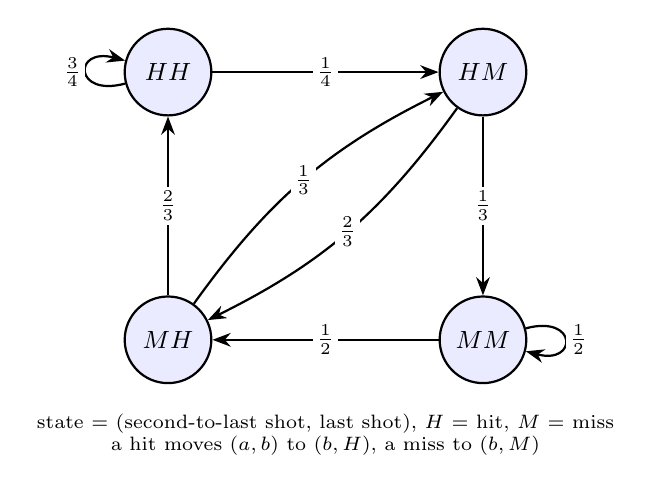
\begin{tikzpicture}[>=Stealth,font=\small,
 s/.style={draw,thick,circle,minimum size=1.1cm,inner sep=0pt,fill=blue!8},
 e/.style={->,thick},
 lab/.style={font=\small,fill=white,inner sep=1.5pt},
 every loop/.style={->,thick,looseness=6}]
\node[s] (HH) at (0,0) {$HH$};
\node[s] (HM) at (4,0) {$HM$};
\node[s] (MH) at (0,-3.4) {$MH$};
\node[s] (MM) at (4,-3.4) {$MM$};
\draw[e] (HH) -- node[lab]{$\tfrac14$} (HM);
\draw[e] (MH) -- node[lab]{$\tfrac23$} (HH);
\draw[e] (HM) -- node[lab]{$\tfrac13$} (MM);
\draw[e] (MM) -- node[lab]{$\tfrac12$} (MH);
\draw[e] (HM) to[bend left=14] node[lab]{$\tfrac23$} (MH);
\draw[e] (MH) to[bend left=14] node[lab]{$\tfrac13$} (HM);
\path (HH) edge[loop left] node[lab]{$\tfrac34$} (HH);
\path (MM) edge[loop right] node[lab]{$\tfrac12$} (MM);
\node[font=\scriptsize,align=center] at (2,-4.6) {state = (second-to-last shot, last shot), $H$ = hit, $M$ = miss\\a hit moves $(a,b)$ to $(b,H)$, a miss to $(b,M)$};
\end{tikzpicture}
\end{document}
